\documentclass[10pt]{article}
\usepackage[utf8]{inputenc}
\usepackage[russian]{babel}
\usepackage[pdftex]{graphicx}
\usepackage{wasysym}
\usepackage{amsmath}
\graphicspath{{.}}
\usepackage{xcolor}
\usepackage{hyperref}
\DeclareGraphicsExtensions{.pdf,.png,.jpg}
\usepackage{geometry} % Меняем поля страницы
\geometry{left=2cm}% левое поле
\geometry{right=3cm}% правое поле
\geometry{top=1cm}% верхнее поле
\geometry{bottom=1.5cm}% нижнее поле
\usepackage{array}
\newcolumntype{P}[1]{>{\centering\arraybackslash}p{#1}}

\begin{document}

\begin{titlepage}

\Large

\begin{center}

Санкт-Петербургский политехнический университет \\ Петра Великого \\
Физико-механический институт \\
Высшая школа прикладной математики и вычислительной
физики

\vspace{6em}

Отчет по лабораторной работе №3\\
по дисциплине\\
"Интервальный анализ"\\

\vspace{2em}

\textbf{Обработка константы}\\

\end{center}


\vspace{5em}

\newbox{\lbox}
\savebox{\lbox}{\hbox{Кромачев Максим Александрович}}

\newlength{\maxl}
\setlength{\maxl}{\wd\lbox}

\hfill\parbox{12cm}{
\hspace*{3cm}\hspace*{-5cm}\hfill\hbox to\maxl{ \hfill}\\
\vspace{0.5em}
\hspace*{3cm}\hspace*{-5cm}\hfill\hbox to\maxl{Выполнил студент: \hfill}\\
\hspace*{3cm}\hspace*{-5cm}\hfill\hbox to\maxl{Кромачев Максим Александрович\hfill}\\
\hspace*{3cm}\hspace*{-5cm}\hfill\hbox to\maxl{группа: 5030102/10201\hfill}\\

\vspace{0.5em}

\hspace*{3cm}\hspace*{-5cm}\hfill\hbox to\maxl{Проверил:}\\
\hspace*{3cm}\hspace*{-5cm}\hfill\hbox to\maxl{доцент}\\
\hspace*{3cm}\hspace*{-5cm}\hfill\hbox to\maxl{Баженов Александр Николаевич}\\
}


\vspace{\fill}

\begin{center}

Санкт-Петербург \\2024

\end{center}

\end{titlepage}

\tableofcontents\newpage

\section{Теоретическое обоснование}
\textbf{Необходимые формулы:}
\begin{itemize}
\item Выборочная медиана
 \begin{equation*}
 med \text{ } x=\begin{cases}
    x_{(l+1)}      & \quad \text{при } n = 2l+1 \\
    \frac{x_{(l)}+x_{(l+1)}}{2} & \quad \text{при } n = 2l
  \end{cases}
 \end{equation*}

\item Ширина интервала:
\begin{equation}
    \text{wid} = \overline{a} - \underline{a}, \quad \text{где } [\underline{a}, \overline{a}] \text{ — интервал}.
\end{equation}

\item Середина интервала:
\begin{equation}
    \text{mid} = \frac{\underline{a} + \overline{a}}{2}, \quad \text{где } [\underline{a}, \overline{a}] \text{ — интервал}.
\end{equation}

\item Радиус интервала:
\begin{equation}
    \text{rad} = \frac{\text{wid}}{2} = \frac{\overline{a} - \underline{a}}{2}.
\end{equation}

\item Минимум по включению:
\begin{equation}
    a \wedge b := \inf \subseteq \{ a, b \} = [\max\{\underline{a}, \underline{b}\}, \min\{\overline{a}, \overline{b}\}] \\
\end{equation}

\item Максимум по включению:
\begin{equation}
    a \wedge b := \sup \subseteq \{ a, b \} = [\min\{\underline{a}, \underline{b}\}, \max\{\overline{a}, \overline{b}\}] \\
\end{equation}


 \item \textit{Модой} интервальной выборки назовём совокупность интервалов пересечения наибольших совместных подвыборок рассматриваемой выборки.
 Пусть имеется интервальная выборка

  \[
    \mathbf{X} = \{ \mathbf{x}_i \}.
  \]

  Сформируем массив интервалов \( \mathbf{z} \) из концов интервалов
  \( \mathbf{X} \).

  Для каждого интервала \( \mathbf{z}_i \) подсчитываем число \( \mu_i \)
  интервалов из выборки \( \mathbf{X}_i \), включающих \( \mathbf{z}_i \).
  Максимальные \( \mu_i = \max \mu \) достигаются для индексного множества
  \( K \). Тогда можно найти интервальную моду как мультиинтервал

  \begin{equation*}
    \text{mode } \mathbf{X} = \bigcup_{k \in K} \mathbf{z}_k.
  \end{equation*}

 \item \textit{Интервальная медиана Крейновича}\\

   Пусть дана выборка \( \mathbf{X} = \{ \mathbf{x}_i \} \). Пусть
  \( \underline c = \{ \underline{\mathbf{x}}_i \} \),
  \( \overline c = \{ \overline{\mathbf{x}}_i \} \) --- конфигурация
  точек, составленные, соответственно, из левых и правых концов интервалов
  из \( \mathbf{X} \).

  Тогда медианой Крейновича \( \text{med}_K \mathbf{X} \) интервальной
  выборки \( \mathbf{X} \) --- это интервал

  \begin{equation*}
    \text{med}_K = [\text{med } \underline c, \text{med } \overline c].
  \end{equation*}

Сложность вычисления \( \text{med}_k X \) составляет \( O(N) \). При определении медианы для интервальных данных мы руководствуемся принципом соответствия. Этот принцип можно сформулировать так: если ширина интервалов стремится к нулю, то значения медианы, рассчитанные для интервальных данных, будут приближаться к значениям медианы для точечных данных, к которым стремятся эти интервалы.

 \item \textit{Интервальная медиана Пролубникова}\\

Для того, чтобы распространить определение медианы точечных данных на интервальные данные, требуется задать для них линейный порядок \( (\leq) \) и частоту. Возможные способы задания отношения порядка на \( \mathbb{IR} \) определены стандартом 1788 IEEE. Говорят, что неравенство \( (\mathbf{a} \leq \mathbf{b}) \) выполняется:

\begin{enumerate}
    \item в сильном смысле, если \( (\forall a \in \mathbf{a})(\forall b \in \mathbf{b})(a \leq b) \);
    \item в слабом смысле, если \( (\exists a \in \mathbf{a})(\exists b \in \mathbf{b})(a \leq b) \);
    \item в \( \forall \exists \)-смысле, если \( (\forall a \in \mathbf{a})(\exists b \in \mathbf{b})(a \leq b) \);
    \item в \( \exists \forall \)-смысле, если \( (\exists a \in \mathbf{a})(\forall b \in \mathbf{b})(a \leq b) \);
    \item в центральном смысле, если \( \frac{\underline{a} + \overline{a}}{2} \leq \frac{\underline{b} + \overline{b}}{2} \).
\end{enumerate}

  Для элементов выборки \( \mathbf{\tilde{X}} \), сформированной на основе выборки \( X = \{ x_i \}_{i=1}^{N} \) и содержащей данные с интервальными неопределённостями, возникшими в результате группировки, можно определить линейный порядок, используя любое из пяти вышеуказанных отношений порядка на \( \mathbb{IR} \). То есть, если \( i \neq j \), то либо \( \tilde{x}_i \leq \tilde{x}_j \), либо \( \tilde{x}_i \geq \tilde{x}_j \) для любого из этих отношений порядка. Это позволяет рассматривать множество \( \mathbf{\tilde{X}} \) для сгруппированных данных как интервальный вариационный ряд.

  Медиана Пролубникова \( \text{med}_P \mathbf{X} \) выборки
  \( \mathbf{X} \) --- это интервал \( \mathbf{x}_m \), для которого
  половина интервалов из \( \mathbf{X} \) лежит слева, а половина
  --- справа.

  В ситуации, когда имеются два элемента подинтервала \( \mathbf{x}_m \)
  и \( \mathbf{x}_{m+1} \), расположенных посередине вариационного ряда,
  \( \mathbf{x}_m \ne \mathbf{x}_{m+1} \) медиана может быть определена
  естественным обобщением взятия полусуммы точечных значений,
  расположенных посередине ряда из точечных значений, в случае
  интервальной выборки взятие полусуммы интервалов \( \mathbf{x}_m \)
  и \( \mathbf{x}_{m+1} \):
    \begin{equation*}
    \text{med}_P \mathbf{X} = (\mathbf{x}_m + \mathbf{x}_{m+1}) / 2.
  \end{equation*}
\item \textit{Коэффициент Жаккара}:\\
 Коэффициент Жаккара для двух интервалов \( \mathbf{x} \in \mathbb{IR} \)
  и \( \mathbf{y} \in \mathbb{IR} \):

  \begin{equation*}
    \text{Ji} (\mathbf{x}, \mathbf{y})
      = \frac{\text{wid} (x \land y)}{\text{wid} (x \lor y)}
      = \frac{\min \{ \overline{\mathbf{x}}, \overline{\mathbf{y}} \} - \max \{ \underline{\mathbf{x}}, \underline{\mathbf{y}} \}}
        {\max\{ \overline{\mathbf{x}}, \overline{\mathbf{y}} \} - \min \{ \underline{\mathbf{x}}, \underline{\mathbf{y}} \}}.
  \end{equation*}

  Коэффициент Жаккара для множества интервалов
  \( \mathbf{X} \in \mathbb{IR}^n \):

  \begin{equation*}
    \text{Ji} (\mathbf{X})
      = \frac{\min \overline{\mathbf{x}_i} - \max \underline{\mathbf{x}_i}}
        {\max \overline{\mathbf{x}_i} - \min \underline{\mathbf{x}_i}}.
  \end{equation*}

  Коэффициент Жаккара для двух множеств интервалов
  \( \mathbf{X} \in \mathbb{IR}^n \) и \( \mathbf{Y} \in \mathbb{IR}^n \):

  \begin{equation*}
    \text{Ji}_k (\mathbf{X}, \mathbf{Y})
      = \frac{\min \{ \overline{\mathbf{x}_k}, \overline{\mathbf{y}_k} \} - \max \{ \underline{\mathbf{x}_k}, \underline{\mathbf{y}_k} \}}
        {\max\{ \overline{\mathbf{x}_k}, \overline{\mathbf{y}_k} \} - \min \{ \underline{\mathbf{x}_k}, \underline{\mathbf{y}_k} \}},
      \ k \in 1, 2, \dots, |\mathbf{X}|.
  \end{equation*}
\end{itemize}
\vspace{0.5cm}

\section{Постановка задачи}
Даны 2 интервальных выборки
\begin{equation}
    \mathbf{X}=\{x_i\},
\end{equation}
\begin{equation}
    \mathbf{Y}=\{y_k\},
\end{equation}
Взять $\mathbf{X}$, $\mathbf{Y}$ из файлов данных, задав rad $x$ = rad $y$ = $\frac{1}{2^N}$, N=14.
Файлы данных:
\[−0.205\_lvl\_side\_a\_fast\_data.bin\]
\[0.227\_lvl\_side\_a\_fast\_data.bin\]
Формат файлов — Save to BIN.pdf.\\
Связь кодов данных и В:\\
\[V = Code/16384 − 0.5.\]
Сделать оценки констант $a$, $t$ в уравнениях.
\begin{equation}
    a+\mathbf{X}=\mathbf{Y},
\end{equation}
\begin{equation}
    t*\mathbf{X}=\mathbf{Y},
\end{equation}
Метод решения:

\begin{equation}
    \hat a = \text{argmax} F(a, \mathbf{X}, \mathbf{Y}),
\end{equation}
где \( F \) --- функционал.
\\
В качестве функционала взять варианты:

  \begin{equation} \label{eq:F_1}
    \text{Ji} (a, \mathbf{X}, \mathbf{Y}),
  \end{equation}
  \begin{equation} \label{eq:F_2}
    \text{Ji} (a, \text{mode} \mathbf{X}, \text{mode} \mathbf{Y}),
  \end{equation}
  \begin{equation} \label{eq:F_3}
    \text{Ji} (a, \text{med}_K \mathbf{X}, \text{med}_K \mathbf{Y}),
  \end{equation}
  \begin{equation} \label{eq:F_4}
    \text{Ji} (a, \text{med}_P \mathbf{X}, \text{med}_P \mathbf{Y}),
  \end{equation}
где \( \text{Ji} \) --- коэффициент Жаккара, \( \text{mode} \) --- интервальная мода, \( \text{med}_K \), \( \text{med}_P \) --- интервальные медианы Крейновича и Пролубникова.\\
Сделать точечные и интервальные оценки, задавшись уровнем \( \alpha \).


\section{Описание работы}

Лабораторная работа выполнена на языке программирования Python в среде разработки VSCode. В ходе работы были использованы следующие библиотеки: numpy, intvalpy, pandas. GitHub репозиторий: \url{https://github.com/kromachmax/Intervalka}

\section{Описание алгоритма}

Для поиска максимума функционалов будем использовать метод дихотомии для интервала, где функционал унимодален\\
\textbf{Вход:}
\\$f(x)$-унимодальная на $[a_0,b_0]$ функция;
\\$a_0$, $b_0$ - крайние точки интервала неопределенности;
\\$\varepsilon$ - точность, с которой необходимо найти максимум функции $f(x)$
\\
\textbf{Выход:}
\\$x_*$ - точка максимума функции $f(x)$;
\\$f(x_*)$ - значение функции $f(x)$ в точке максимума




\section{Результаты}
Дальше в таблице $const$ - это константа, для которой ищем оценку.\\
Возъмём уровень $\alpha=0.001$

\begin{center}
\begin{tabular}{|c|c|c|}
\hline
\multicolumn{3}{|c|}{$\text{Ji} (a/t, \mathbf{X}, \mathbf{Y})$ }\\
\hline
const&Оценка&Значение функционала\\
\hline
$\hat{a}$&$ 0.3409\pm0.001$&-0.7867\\
\hline
$\hat{t}$&$-1.0502\pm0.001$&-0.8610\\
\hline
\hline
\multicolumn{3}{|c|}{$\text{Ji} (a/t, \text{mode} \mathbf{X}, \text{mode} \mathbf{Y})$ }\\
\hline
const&Оценка&Значение функционала\\
\hline
$\hat{a}$&$0.3402\pm0.001$&-0.25437\\
\hline
$\hat{t}$&$-0.9987\pm0.001$&-0.92750\\
\hline
\hline
\multicolumn{3}{|c|}{$\text{Ji} (a/t, \text{med}_K \mathbf{X}, \text{med}_K \mathbf{Y})$}\\
\hline
const&Оценка&Значение функционала\\
\hline
$\hat{a}$&$0.3436\pm0.001$&0.1351\\
\hline
\hline
$\hat{t}$&$-1.0144\pm0.001$&0.7746\\
\hline
\multicolumn{3}{|c|}{$\text{Ji} (a/t, \text{med}_P \mathbf{X}, \text{med}_P \mathbf{Y})$}\\
\hline
const&Оценка&Значение функционала\\
\hline
$\hat{a}$&$0.3436\pm0.001$&0.1351\\
\hline
$\hat{t}$&$-1.0144\pm0.001$&0.7746\\
\hline
\end{tabular}
\end{center}\\


\newpage
\subsection{Графики}
\\Продемонстрируем результаты вычислений на графиках.
\begin{figure}[h!]
    \centering
    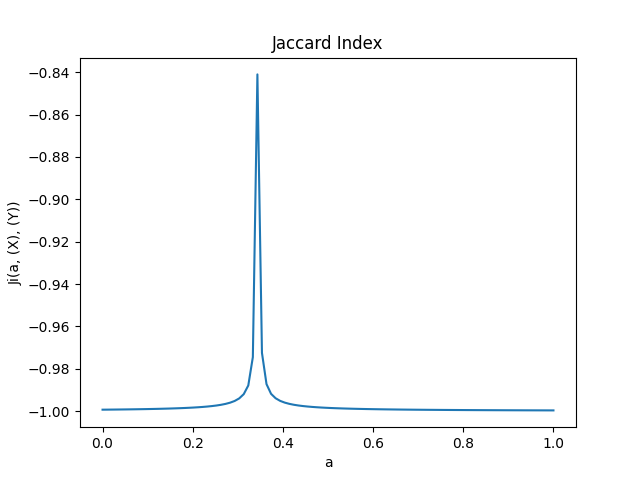
\includegraphics[width=0.75\linewidth]{Jaccadrd-a-.png}
    \caption{Коеффициент Жаккара для a, функционал (6)}
\end{figure}
\begin{figure}[h!]
    \centering
    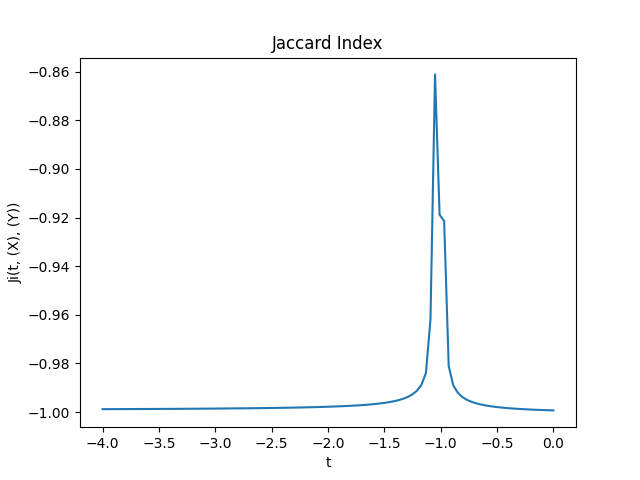
\includegraphics[width=0.75\linewidth]{Jaccadrd-t-.png}
    \caption{Коеффициент Жаккара для t, функционал (6)}
\end{figure}

\newpage
\begin{figure}[h!]
    \centering
    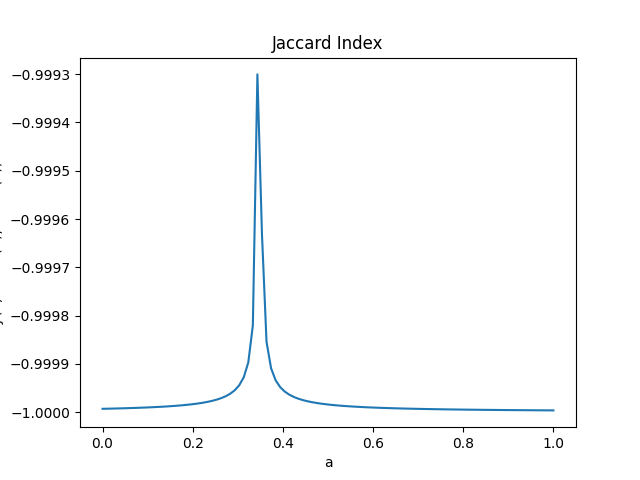
\includegraphics[width=0.75\linewidth]{Jaccadrd-a-mode.png}
    \caption{Коеффициент Жаккара для a, функционал (7)}
\end{figure}

\begin{figure}[h!]
    \centering
    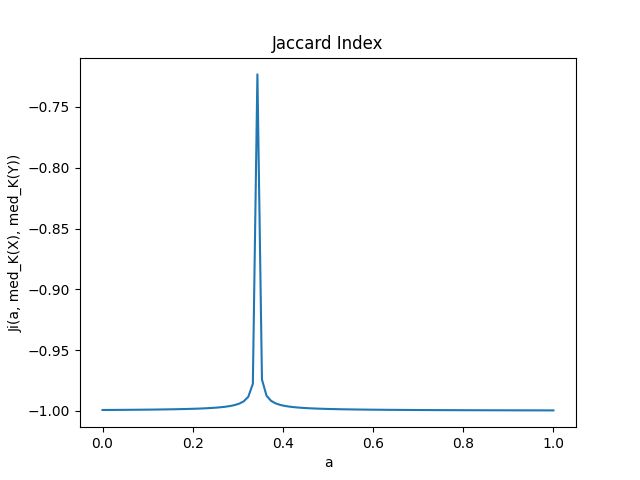
\includegraphics[width=0.75\linewidth]{Jaccadrd-a-med_K.png}
    \caption{Коеффициент Жаккара для a, функционал (8)}
\end{figure}

\newpage
\begin{figure}[h!]
    \centering
    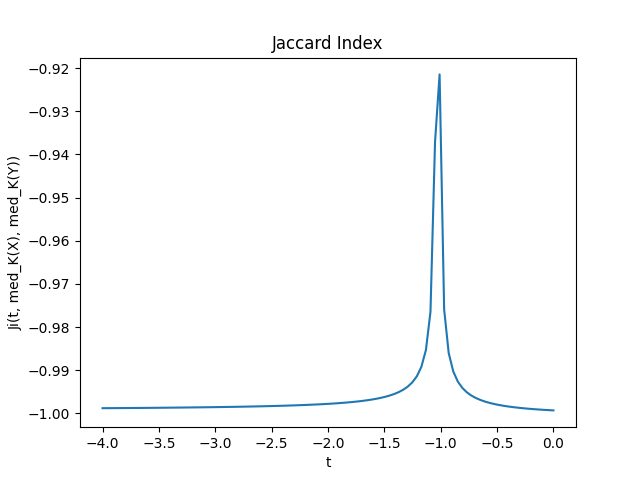
\includegraphics[width=0.75\linewidth]{Jaccadrd-t-med_K.png}
    \caption{Коеффициент Жаккара для t, функционал (8)}
\end{figure}

\begin{figure}[h!]
    \centering
    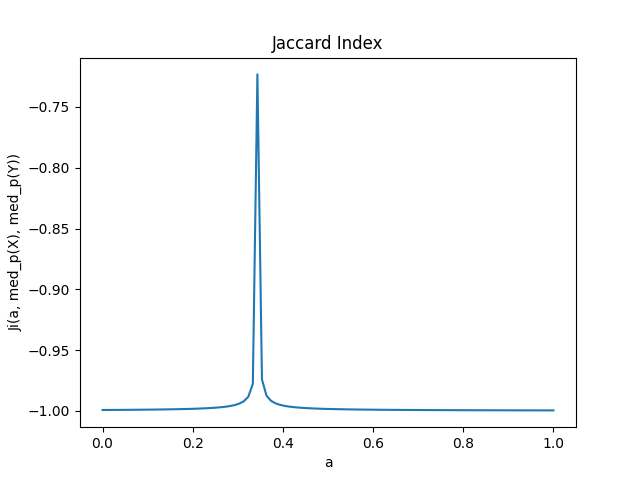
\includegraphics[width=0.75\linewidth]{Jaccadrd-a-med_p.png}
    \caption{Коеффициент Жаккара для a, функционал (9)}
\end{figure}

\newpage
\begin{figure}[h!]
    \centering
    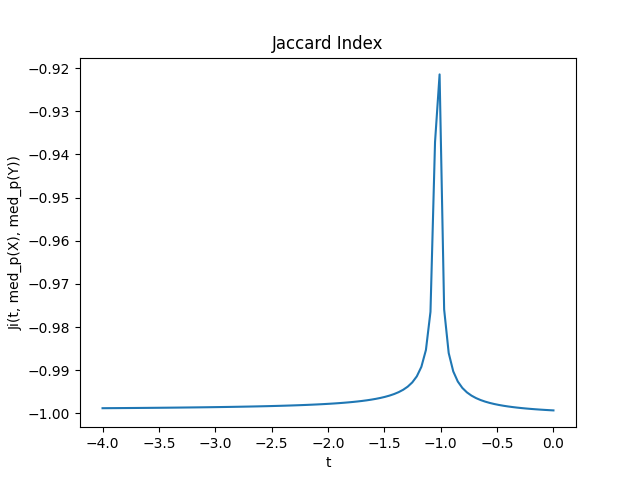
\includegraphics[width=0.75\linewidth]{Jaccadrd-t-med_p.png}
    \caption{Коеффициент Жаккара для t, функционал (9)}
\end{figure}

\section{Итоги}

В процессе выполнения лабораторной работы мы ознакомились с методами получения интервальных оценок для констант. Фокусировались на четырех различных функционалах ((6), (7), (8), (9)), основанных на вычислении коэффициента Жаккара, но применяемых к различным интервальным множествам.

Мы пришли к следующим выводам:

\begin{enumerate}
    \item Важно тщательно подбирать функционал для поиска оценок. Разные функционалы могут приводить к несовместимости интервалов, как это наблюдалось при использовании функционала $Ji(const,\mathbf{X},\mathbf{Y})$. В то же время, для функционалов $\text{Ji} (const, \text{med}_K \mathbf{X}, \text{med}_K \mathbf{Y})$ и $\text{Ji} (const, \text{med}_P \mathbf{X}, \text{med}_P \mathbf{Y})$ интервалы оказались совместимыми.

    \item Можно отметить, что использование функционалов, зависящих от медиан (8), (9), приводит к коэффициенту Жаккара, близкому к 1 (значение 0.7746) для оценки \( t \), что указывает на высокую степень совпадения выборок \( t*\mathbf{X} \) и \( Y \).

    \item В ходе исследования мы также обнаружили, что функционал, зависящий от моды (7), требует значительно больше времени на вычисление оценок по сравнению с другими функционалами. Это свидетельствует о том, что для больших интервальных выборок использование коэффициента Жаккара, основанного на модах (7), нежелательно. Предпочтительнее использовать коэффициент Жаккара, основанный на одной из медиан (Крейновича или Пролубникова).

    \item Кроме того, при нахождении медианы Пролубникова, если мы вводим порядок в алгебре \( \mathbb{IR} \) в центральном смысле (\( (\overline{\mathbf{a}} + \underline{\mathbf{a}}) / 2 \leq (\overline{\mathbf{b}} + \underline{\mathbf{b}}) / 2 \)), оценки, полученные с использованием функционала медианы Крейновича и медианы Пролубникова, совпадают.
\end{enumerate}

\end{document}
